\subsection*{Experiment III}
\begin{frame}{Intervention 1 and 2: Summary}
    \uncover<2->{
        \begin{itemize}
        \item assessments correct workseekers' self-evalution
        \item assessment reports change job searching, especially the \texthlit{certified} ones
        \item assessment reports improve employment and wages, even the \texthlit{un-certified} ones
        
        \uncover<3->{\footnotesize BUT, those experiencing these improvements do \texthlbf{not} use the private assessment reports}
        \end{itemize}
    }
    \vspace*{10pt}
    \uncover<4->{What can we infer?
    \begin{itemize}
        \item<5-> only firm-side learning \textcolor{fuzzywuzzy!65!white}{(\ding{55})}
        \begin{itemize}
            \footnotesize
            \item<6->[W] assessment reports are used, workseekers' beliefs are shifted
            \item<7->[F] survey evidence that hiring managers would \texthlit{not} view the private certificates as credible
        \end{itemize}
        \item<8-> only workseeker-side learning \textcolor{fuzzywuzzy!65!white}{(\ding{55})}
        
        {\footnotesize no significant changes in \textcolor<9>{fuzzywuzzy!65!white}{targeting and search effort}}
    \end{itemize}
    }

\end{frame}

\begin{frame}{Intervention 3: Direct Information Provision to Firms}
    \vspace*{-5pt}
    \begin{itemize}
        \small
        \item[\texthlit{T3}] randomly use 1 or 3 real certified resumes, randomly applying for vacancies
    \end{itemize}
    \begin{table}[h!]
        \small
        \begin{center}
            \begin{tabular}{lccc}
            
            & \multicolumn{2}{c}{{\textbf{report}}} & \multirow{2}{*}{{\textbf{no report}}} \\
            & {\color{fuzzywuzzy!65!white} {\textit{shareable}}} & {\textit{non-shareable}} & \\
            \hline
            \multirow{2}{*}{{\color{fuzzywuzzy!65!white} \underline{No. certified applicants}}} & \multicolumn{2}{c}{\transparent{0.2}?} & {0} \\
             & {{?}} & {\transparent{0.2}?} &
            \end{tabular}
        \end{center}
    \end{table}
\end{frame}

\begin{frame}{Intervention 3: Experiment Procedure}
    \begin{columns}[T]
        \uncover<1->{\begin{column}{0.45\textwidth}
            \begin{block}{\small \centering \textbf{Workseeker}}
                \begin{itemize}
                    \small
                    \item<2-> invite 2220 \textit{assessed} candidates for CVs
                    \item<2-> 717 submissions
                \end{itemize}
            \end{block}
        \end{column}}

        \uncover<1->{\begin{column}{0.45\textwidth}
            \begin{block}{\small \centering \textbf{Jobs}}
                \begin{itemize}
                    \small
                    \item<3-> select 1068 \textit{suitable} vacancies
                    \item<3-> keep 998 vacancies
                \end{itemize}
            \end{block}
        \end{column}}
    \end{columns}

    \uncover<4->{\vspace*{10pt}
        Randomization: \uncover<5>{whether firms get credible information, do they get \textit{overloaded}}
        \begin{center}
            \small
            \begin{tabular}{lcccccc}
           Total & Group & Assessed & \#applications/vacancy & ideal\% & actual\%  \\ \hline
           \multirow{4}{*}{3992{\scriptsize =998$\times$4}} & (1) & \textcolor{fuzzywuzzy!65!white}{Yes} & \textcolor{fuzzywuzzy!65!white}{1} & 1/8 & 12\% \\
            & (2) & No & 1 & 3/8 & 37\% \\
            & (3) & \textcolor{fuzzywuzzy!65!white}{Yes} & \textcolor{fuzzywuzzy!65!white}{3} & 3/8 & 38\% \\
            & (4) & No & 3 & 1/8 & 13\%
            \end{tabular}
        \end{center}
        }
\end{frame}

\begin{frame}{Intervention 3: Estimation on Application Level}
    \begin{align*}
        Y_{rv} = \underbrace{\mathrm{Certificate}_{rv}}_{=\mathbf{1}(\text{public})}\cdot \beta_1 + \mathrm{Certificate}_{rv}\cdot \underbrace{\mathrm{HighIntensity}_{v}}_{=\mathbf{1}(\text{3 applications})}\cdot \beta_2 + \mathbf{V}_v + \mathbf{X}_r\cdot \Gamma + \mathbf{E}_{rv}+\epsilon_{rv}
    \end{align*}
    \begin{itemize}
        \small
        \item $\mathbf{V}_{v}$ vacancy FEs, $\mathbf{X}_{v}$ resume covariates, $\mathbf{E}_{rv}$ email address FEs
    \end{itemize}

    \uncover<2>{\begin{center}
        \footnotesize
        \begin{tabular}{lccccc}
        & \multicolumn{2}{c}{Any repsonse} & & \multicolumn{2}{c}{Interview invitation} \\ \cline{2-3} \cline{5-6}
        & (1) & (2) & & (3) & (4) \\ \hline
       $\beta_1$ & 0.015{ \tiny(0.009)} & 0.016{ \tiny(0.009)} & & 0.009{ \tiny(0.004)} & 0.010{ \tiny(0.006)} \\
       $\beta_2$ & -0.027{ \tiny(0.013)} & -0.028{ \tiny(0.014)} & & -0.016{ \tiny(0.009)} & -0.017{ \tiny(0.010)} \\
       &\\
       mean (C) & \multicolumn{2}{c}{0.130} & & \multicolumn{2}{c}{0.087} \\
       FEs and controls & No & Yes & & No &Yes 
        \end{tabular}
    \end{center}}
\end{frame}

\begin{frame}{Intervention 3: Estimation on Vacancy Level}
    \begin{align*}
        Y_{v} = \underbrace{\mathrm{HighIntensity}_{v}}_{=\mathbf{1}(\text{3 applications})}\cdot \alpha + \eta_v
    \end{align*}

    \uncover<2>{\begin{center}
        \footnotesize
        \begin{tabular}{lccccc}
        & \multicolumn{2}{c}{Repsonse} & & \multicolumn{2}{c}{Interview invitation} \\ \cline{2-3} \cline{5-6}
        & mean & $=\mathbf{1}(\#>0)$ & & mean & $=\mathbf{1}(\#>0)$ \\ \hline
       $\alpha$ & 0.023{ \tiny(0.020)} & \textcolor{fuzzywuzzy!45!white}{0.042{ \tiny(0.026)}} & & -0.001{ \tiny(0.016)} & 0.021{ \tiny(0.021)} \\
       &\\
       mean (C) & 0.134 & 0.187 & & 0.090 & 0.117
        \end{tabular}
    \end{center}}
\end{frame}

\subsection*{Supporting Results}
\begin{frame}{Summary of Intervention 1-3}
    So far: 
    \begin{itemize}
        \small
        \item assessments correct workseekers' self-evalution
        \item assessment reports change job searching, especially the \texthlit{certified} ones
        \item assessment reports improve employment and wages, even the \texthlit{un-certified} ones
        \item \textit{tentatively}, diminishing marginal returns of aggregate certificate use
    \end{itemize}
    
    \vspace*{10pt}
    Firms and workseekers \texthlit{both} learn from the assessment treatment\uncover<2->{, But how?}
    \begin{itemize}
        \small
        \item<3->[A] information channel
        \item<4->[B] signalling channel
        \item<5->[C] behavioral anomalies 
    \end{itemize}
\end{frame}

\begin{frame}{Supporting Result 1: Assessment Results Matter}
    Placebo group (N=254): assessed, reported, certified, \texthlit{without assessment results}
    \begin{center}
        \small
        \begin{tabular}{lcccccc}
        & market & & & & hourly & written \\ 
        & index & employed & hours & earnings & wage & contract \\ \hline
       Public & $0.120^{***}$ & ${0.052^{***}}$ & {$0.201^{***}$} & {$0.337^{***}$} & {$0.197^{***}$} & {$0.020^{**}$} \\
       & \\
       Placebo & \uncover<2>{$0.027$ & $0.020$ & $0.040$ & $0.068$ & $0.053$ & $0.005$ \\
       & $(0.043)$ & $(0.028)$ & $(0.075)$ & $(0.185)$ & $(0.129)$& $(0.021)$ \\
       &\\
       $p_{\text{public=placebo}}$ & ** & & ** & & & }
        \end{tabular}
    \end{center}
\end{frame}

\begin{frame}{Supporting Result 1: Assessment Results Matter}
    Infer \texthlit{WTP}: 69 firms, a standard Decker-DeGroot-Marschak mechanism, on a talent-pool database with the assessment results
    \uncover<2>{
        \begin{figure}
            \centering
            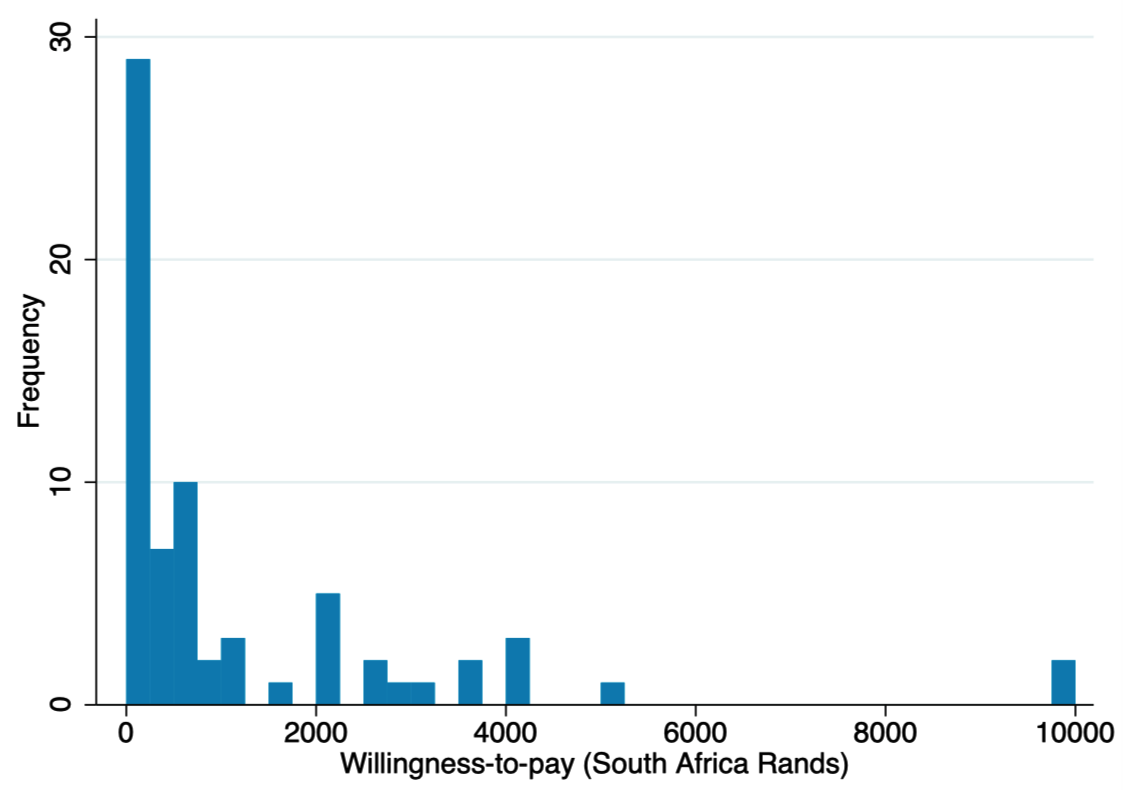
\includegraphics[height = 0.6 \textheight]{images/WTP.png}
        \end{figure}
    }
\end{frame}

\begin{frame}{Supporting Result 2: Horizontal vs Vertical}
    \begin{columns}
        \begin{column}{0.45\textwidth}
            \begin{table}[h!]
                \footnotesize
                \begin{center}
                    \begin{tabular}{lccc}
                    
                    & &\multicolumn{2}{c}{workseekers} \\
                   & & $W_1$ & $W_2$ \\
                    \hline
                    \multirow{2}{*}{jobs} & $J_1$ & $\textcolor{fuzzywuzzy!65!white}{\boxed{V_{1,1}}}$ & $V_{2,1}$ \\
                    & $J_2$ & $V_{1,2}$ & $\textcolor{fuzzywuzzy!65!white}{\boxed{V_{2,2}}}$
                    \end{tabular}
                \end{center}
            \end{table}
            \begin{itemize}
                \footnotesize 
                \item \textcolor{fuzzywuzzy!65!white}{\textbf{horizontal}} differentiation: $$V_{i,i}>V_{i,j},V_{j,j}>V_{j,i}$$
                \item \textcolor{fuzzywuzzy!65!white}{\textbf{vertical}} differentiation: $$V_{i,\cdot}>V_{j,\cdot}$$
            \end{itemize}
        \end{column}
    
        \begin{column}{0.5\textwidth}
            \uncover<2->{{\small no skill-level heterogeneity}
            \begin{center}
                \scriptsize
                \begin{tabular}{lccc}
                & (1) & (2) & (3) \\ \hline
               Public & ${0.052^{***}}$ & ${0.052^{***}}$ & ${0.053^{***}}$\\
               $\times$ TmB & 0.019 \\
               $\times$ PC1(Scores) & & 0.004 \\
               $\times$ w. Scores & & & -0.007
                \end{tabular}
            \end{center}
            }
            \uncover<3>{
                \vspace*{5pt}
                {\small dispersion of \underline{wages $\mid$ employed} doesn't increase}
                \begin{itemize}
                    \footnotesize
                    \item standard deviation: $+0.03$ $\textcolor{fuzzywuzzy!65!white}{(p=0.87)}$
                    \item interquartile range: $+0.65$ $\textcolor{fuzzywuzzy!65!white}{(p=0.57)}$
                    \item interdecile range: $+0.42$ $\textcolor{fuzzywuzzy!65!white}{(p=0.41)}$
                \end{itemize}
            }
            
        \end{column}
    \end{columns}
\end{frame}

\begin{frame}{Supporting Result 2: Horizontal vs Vertical}
    \vspace*{-10pt}
    \begin{columns}[T]
        \begin{column}{0.45\textwidth}
            \begin{figure}
                \centering
                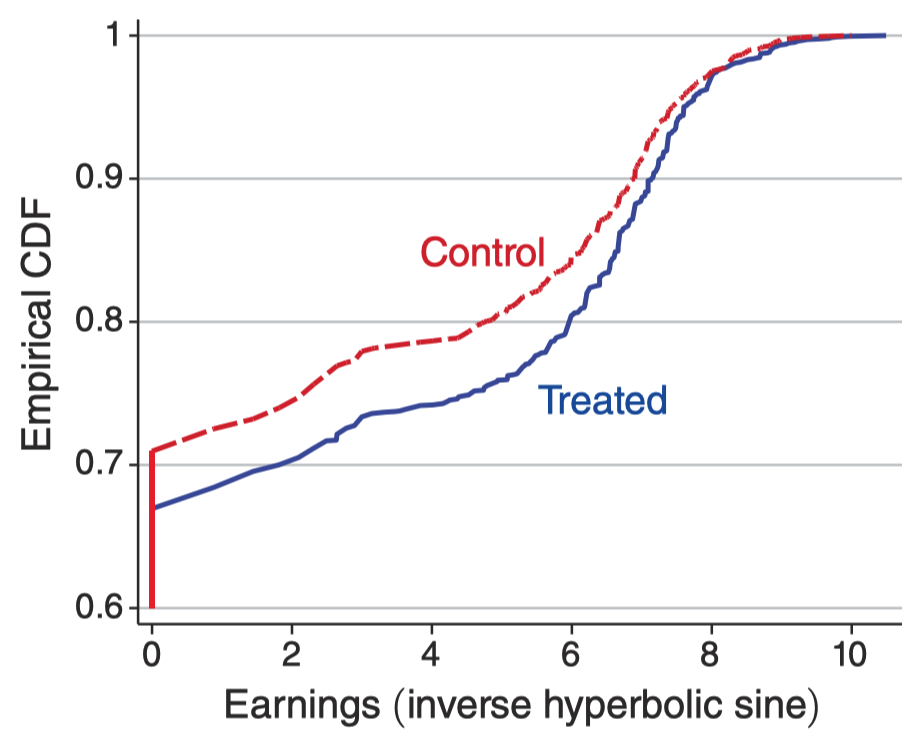
\includegraphics[height = 0.6 \textheight]{images/dist_earnings.png}
            \end{figure}
        \end{column}

        \begin{column}{0.45\textwidth}
            \begin{figure}
                \centering
                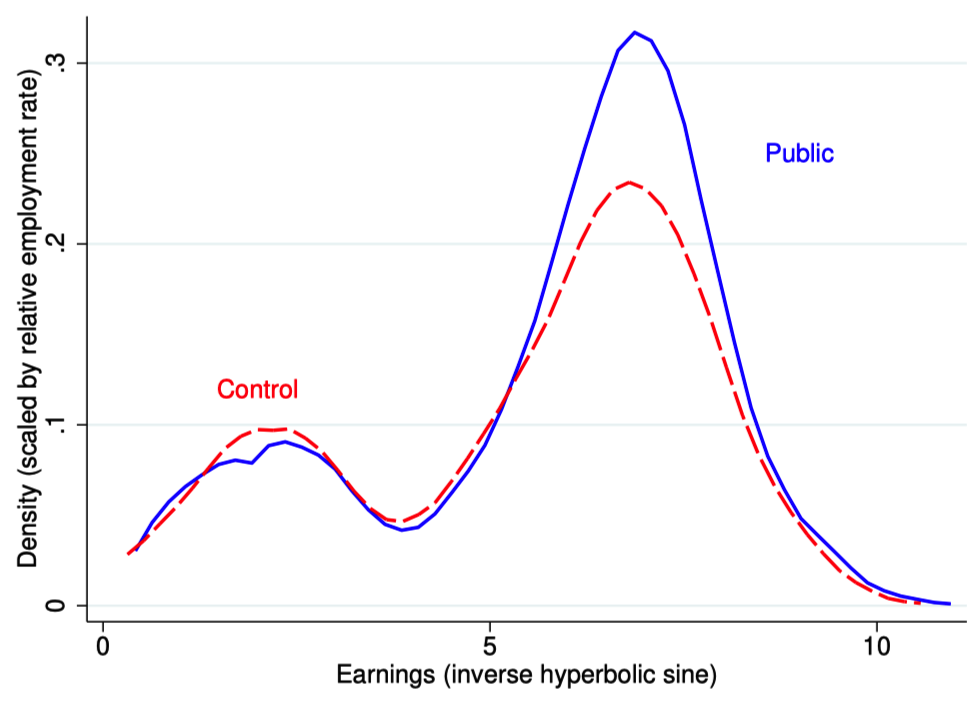
\includegraphics[height = 0.6 \textheight]{images/dist_earnings_empadj.png}
            \end{figure}
        \end{column}
    \end{columns}
\end{frame}

\begin{frame}{Supporting Result 2: Horizontal vs Vertical}
    \begin{itemize}
        \item<+-> The 6 assessments are \texthlit{weakly correlated}
        \item<+-> workseekers with different skills respond differently to the treatment
        \begin{itemize}
            \item[-] high skilled workseekers more likely to \texthlit{use certificates}
            \item[-] low skilled workseekers more likely to engage in \texthlit{search targeting} 
        \end{itemize} 
        \item<+-> firms' relative demand for different skills is heterogeneous 
    \end{itemize}

    \only<1>{
        \begin{table}[h!]
            \footnotesize
            \begin{center}
                \begin{tabular}{rccccc}
                    & concept formation & grit & numeracy & focus & \texthlit{planning} \\ \hline
                    communication & 0.346 & 0.088 & 0.393 & 0.171 & 0.258 \\
                    concept formation && 0.094 & 0.519 & 0.225 & 0.292\\
                    grit & && 0.128 & 0.049 & 0.106\\
                    numeracy &&&& 0.162 & 0.325 \\
                    \texthlit{focus} &&&&&0.181
                \end{tabular}
            \end{center}
        \end{table}
    }

    \only<3>{
        \begin{table}[h!]
            \footnotesize
            \begin{center}
                \begin{tabular}{rc|ccc}
                in top tecile & education & ranked first & ranked last & median rank \\
                \hline
                communication & secondary & 0.119 & 0.015 & 3 \\
                concept formation & secondary & 0.075 & 0.030 & 4 \\
                focus & secondary & 0.328 & 0.060 & 3 \\
                grit & secondary & 0.134 & 0.045 & 4 \\
                numeracy & secondary& 0.060 & 0.090 & 2  \\
                planning & secondary& 0.194 & 0.000 & 4\\
                none & 1-year post-secondary & 0.000 & 0.761 & 7
                \end{tabular}
            \end{center}
        \end{table}
    }
\end{frame}

\begin{frame}{Supporting Result 3: Certification Mitigates Limited Information}
    \begin{center}
        \small
        \begin{tabular}{lccc}
        & (1) & (2) & (3) \\ \hline
       Public & ${0.051^{***}}$ & ${0.052^{***}}$ & ${0.051^{***}}$\\
        &\\
       $\times$ post-secondary education & $-0.028$ \\
       & $(0.028)$\\
       $\times$ employed at baseline & & $-0.043$ \\
       & & $(0.032)$ \\
       $\times \hat{\Pr}\left(\text{Employed at endline}\mid \mathbf{X}\right)^1$  & & & $-0.076^{***}$ \\ % the treatment substitutes the tranditional sources of information, even out undesirable differences
       && & $(0.028)$\\ \hline
       \multicolumn{4}{l}{\footnotesize estimated with baseline variables, following Abadie et al. (2018)}
        \end{tabular}
    \end{center}
\end{frame}